%%%%%%%%%%%%%%%%%%%%%%%%%%%%%%%%%%%%%%%%%
% Formal Book Title Page
% LaTeX Template
% Version 2.0 (23/7/17)
%
% This template was downloaded from:
% http://www.LaTeXTemplates.com
%
% Original author:
% Peter Wilson (herries.press@earthlink.net) with modifications by:
% Vel (vel@latextemplates.com)
%
% License:
% CC BY-NC-SA 3.0 (http://creativecommons.org/licenses/by-nc-sa/3.0/)
% 
% This template can be used in one of two ways:
%
% 1) Content can be added at the end of this file just before the \end{document}
% to use this title page as the starting point for your document.
%
% 2) Alternatively, if you already have a document which you wish to add this
% title page to, copy everything between the \begin{document} and
% \end{document} and paste it where you would like the title page in your
% document. You will then need to insert the packages and document 
% configurations into your document carefully making sure you are not loading
% the same package twice and that there are no clashes.
%
%%%%%%%%%%%%%%%%%%%%%%%%%%%%%%%%%%%%%%%%%

%----------------------------------------------------------------------------------------
%	PACKAGES AND OTHER DOCUMENT CONFIGURATIONS
%----------------------------------------------------------------------------------------

\documentclass[a4paper, 11pt, oneside]{article} % A4 paper size, default 11pt font size and oneside for equal margins

\newcommand{\plogo}{\fbox{$\mathcal{PL}$}} % Generic dummy publisher logo

\usepackage[utf8]{inputenc} % Required for inputting international characters
\usepackage[T1]{fontenc} % Output font encoding for international characters
\usepackage{fouriernc} % Use the New Century Schoolbook font
\usepackage{graphicx} 
\usepackage[hmarginratio=1:1,top=25mm,columnsep=20pt,total={6in, 9in}]{geometry}
\usepackage{tocloft}
\usepackage{booktabs}
\usepackage{pdfpages} 
\usepackage{float}
\usepackage{siunitx}
\usepackage{ragged2e}
\usepackage{fancyhdr}
\usepackage{subfig}
%\usepackage{nomencl}
%\makenomenclature
%\renewcommand{\nompreamble}{This list describes several symbols that will be later used within this thesis}
 
\pagestyle{fancy}
\fancyhf{}
\rhead{B.J. Norfolk}
\lhead{Final Year Thesis}
\cfoot{\thepage}
%\usepackage[style=numeric,natbib]{biblatex}
%\addbibresource{sample.bib} 
%----------------------------------------------------------------------------------------
%	TITLE PAGE
%----------------------------------------------------------------------------------------

\begin{document} 

\begin{titlepage} % Suppresses headers and footers on the title page

	\centering % Centre everything on the title page
	
	\scshape % Use small caps for all text on the title page
	
	\vspace*{1\baselineskip} % White space at the top of the page
	
	%------------------------------------------------
	%	Title
	%------------------------------------------------
	\begin{figure}[H] 
	 \centering
	 
\includegraphics[scale=0.4]{monash_logo.jpg} 
    \end{figure}
    Department of Mechanical and Aerospace Engineering
    
    \vspace{2\baselineskip}
    
	{\Large Honours Thesis}
	

	\vspace{2cm}
	
	\rule{\textwidth}{1.6pt}\vspace*{-\baselineskip}\vspace*{2pt} % Thick horizontal rule
	\rule{\textwidth}{0.4pt} % Thin horizontal rule
	
	\vspace{1.5\baselineskip} % Whitespace above the title
	
	{\LARGE Transient Supersonic Jets} % Title
	
	\vspace{1.5\baselineskip} % Whitespace below the title
	
	\rule{\textwidth}{0.4pt}\vspace*{-\baselineskip}\vspace{3.2pt} % Thin horizontal rule
	\rule{\textwidth}{1.6pt} % Thick horizontal rule
	
	\vspace{2\baselineskip} % Whitespace after the title block
	
	%------------------------------------------------
	%	Subtitle
	%------------------------------------------------
	

	
	\vspace*{3\baselineskip} % Whitespace under the subtitle
	
	%------------------------------------------------
	%	Editor(s)
	%------------------------------------------------
	
	Author
	
	\vspace{0.5\baselineskip} % Whitespace before the editors
	
	{\scshape\Large Brodie James Norfolk} % Editor list
	
	\vspace{2\baselineskip}
	Supervisor
	
	\vspace{0.5\baselineskip} % Whitespace before the editors
	
	{\scshape\Large Daniel Edgington-Mitchell} % Editor list
	
	\vspace{2\baselineskip} % Whitespace below the editor list
	
	 % Editor affiliation
	
	\vfill % Whitespace between editor names and publisher logo
	
	\begin{figure}[H] 
	 \centering
	 
\includegraphics[scale=0.6]{ltrac_logo.png} 
    \end{figure}
	
	%------------------------------------------------
	%	Publisher
	%------------------------------------------------
	


\end{titlepage}
\pagenumbering{roman}
\section*{Abstract}
This thesis aims to explore the fundamental fluid dynamics for transient supersonic jets by means of varying the exit flow nozzle geometry and introducing an impingement plate set at $90^{\circ}$ to the oncoming flow. The study of transient supersonic jets has applications in pressure gain combustion (PGC). PGC is a constant volume combustion process applicable to gas turbines that operates by increasing the stagnation pressure entering the turbine via heat released from combustion. Increasing the turbine inlet pressure allows for considerably more work to be extracted when the turbine expands the flow back to the free stream pressure. The unique design presented in PGC engines predicts 
possible advances in thermodynamic efficiencies leading to significantly lower fossil fuel consumption. The experiment undertaken compares flow regimes of NUMBER and NUMBER Mach numbers for each nozzle geometry at impingement plate positions of LENGTH and LENGTH inner nozzle diameters. Transient jet impingement has previously been studied, although it is absent of extensive, repeated experiments, high quality schlieren, and variable exit geometry. This thesis aims to address absences in the literature and explore in detail the shock-vortex interaction during jet impingement. The fundamental fluid dynamics under investigation are; nozzle geometry effects on the shock-vortex interaction and jet impingement, and Mach number variations on all of the latter. 
\newpage
\section*{Acknowledgements}
The author would like to thank those who provided advice and guidance throughout this project. Particularly Dr. Daniel Edgington-Mitchell who supervised the year long project and gave integral feedback, and Bhavraj Thethy for working tirelessly to prepare a functioning laboratory and contributing useful discussions. The author also wishes to acknowledge fellow undergraduate and graduate students including Thomas Knast, Sam Lock, Anesu Junior Kusangaya, and Marcus Wong for assisting in laboratory development and providing key suggestions.
\newpage
\tableofcontents
\newpage
\listoftables
\newpage
\listoffigures
\newpage
\section*{Nomenclature}
%This list describes several symbols that will be later used within this thesis.
%\mbox{}
\begin{table}[H]
\begin{tabular}{ll} \smallskip
$M_1$      & Ambient Mach number                         \\ \smallskip
$P_1$      & Ambient pressure, Pa                        \\ \smallskip
$P_4$      & Shock tube driver section pressure, Pa      \\ \smallskip
$U_1$      & Ambient air velocity, m/s                   \\ \smallskip
$U_4$      & Shock tube driver section air velocity, m/s \\ \smallskip
$\gamma_1$ & Ambient specific heat ratio                 \\ \smallskip
$\gamma_4$ & Driver specific heat ratio                 
\end{tabular}
\end{table}
%\nomenclature{$M_1$}{Ambient Mach number}
%\nomenclature{$P_1$}{Ambient pressure, Pa}
%\nomenclature{$P_4$}{Shock tube driver section pressure, Pa}
%\nomenclature{$U_1$}{Ambient air velocity, m/s}
%\nomenclature{$U_4$}{Shock tube driver section air velocity, m/s}
%\nomenclature{$\gamma_1$}{Ambient specific heat ratio}
%\nomenclature{$\gamma_4$}{Driver specific heat ratio}
 
%\printnomenclature


\newpage
\pagenumbering{arabic}
\section{Introduction} 

\subsection{Motivation}
Understanding transient supersonic jets is integral for the integration of pressure gain combustion in ground and aerospace gas turbine applications. PGC offers a significant gain in thermodynamic efficiencies and subsequent reduction in fossil fuel consumption. The literature adeptly describes transient supersonic jet fluid dynamics for propagation from a no nozzle shock tube, and impingement on plates set to varying angles in respect to the flow. However, there is an absence of extensive, repeated experiments, high quality schlieren, and variable exit geometry. The motivation of this experiment is to address  absences in the literature discussed in \ref{sec:background} and to explore in detail, the shock-vortex interaction during jet impingement. To this end the project will seek to answer the following research questions:

\subsection{Aims}
This thesis aims to explore the fundamental fluid dynamics for transient supersonic jets by means of varying the exit flow nozzle geometry and introducing an impingement plate set at $90^{\circ}$ to the oncoming flow. The propagation and time dependent growth of transient and trailing jet Mach disks will be investigated in an attempt to address absences in the literature, and explore in detail the shock-vortex interaction during jet impingement. The pixel relative velocity of the impinging shock wave for plate and no plate experiments will be extracted from the data in order to define each individual flow regime. The fundamental fluid dynamics under investigation are; nozzle geometry effects on the shock-vortex interaction and jet impingement, and Mach number variations on all of the latter.


\newpage

\section{Background Theory} \label{sec:background}
Gas turbine engines are an integral component for the function of ground based power generation and aircraft engines. They account for a large percentage of power generation world wide. Thermodynamic cycle advances in gas turbine design play an important role in preventing the growth of emissions pollution and prolonged global warming \cite{paxson2018pressure}. Pressure gain combustion (PGC) shown in Figure \ref{fig:pcg} is one possible to method of efficiency improvement. PGC is a constant volume combustion process that operates by increasing the stagnation pressure entering the turbine via heat released from combustion. Increasing the turbine inlet pressure allows for considerably more work to be extracted when the turbine expands the flow back to the free stream pressure. PGC optimises gas turbine thermodynamic cycle efficiency, and has the potential to increase current engine efficiency up to 10\% \cite{gulen2013constant}.

\begin{figure}[H] 
 \centering
 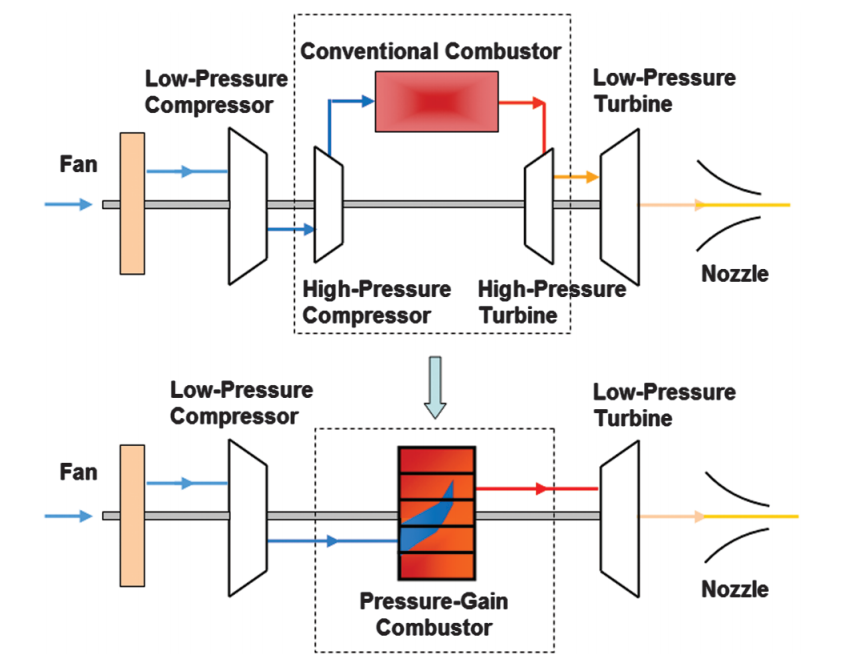
\includegraphics[scale=0.5]{pcg.png} 
 \caption{PCG design concept \cite{akbari2009review}.}
 \label{fig:pcg}
\end{figure}

PGC is at peak efficiency when accomplished through detonation driven combustion, this involves the implementation of detonation waves within the combuster to cause an increase in the temperature and pressure of the fuel-air mixture \cite{eidelman1991review}. During combustion, detonation waves produce flow at supersonic velocities leading to an approximate constant volume and significant pressure gain across the combustor. For supersonic velocities high pressure turbine inlet flow must be steady. A possible method to achieve steady flow at the turbine inlet is via the implementation of a pulse detonation engine \cite{kailasanath2009research} with an equalising plenum chamber. Wear on the first stage of the turbine presents itself as one of the most significant problems of PGC implemetation in current engines. Replacing the combustor in a conventional gas turbine with a pulse detonation combustor (PDC) will result in the propergating detonation waves to converge on the first stage of the turbine. This overtime can lead to concentrated wear on the first stage of the turbine high wear stress points \cite{dean2005operation}. To alleviate turbine wear, the utilization of a high pressure plenum chamber is placed at the exit of the PDC, and creates steady flow conditions effectively shielding the first stage of the turbine from combustion detonations. It remains unclear on how to integrate a pressure plenum into a PDC design. 

The fluid dynamics characterising the governing flow at the exit of PDC is defined as a shock-driven, transient, supersonic jet process \cite{radulescu2007transient}. The governing flow can be classified into several different stages \cite{ishii1999experimental} as shown in Figure \ref{fig:0}. The first stage of jet evolution is defined by the diffraction of a shock wave around the corners of the tube exit, this region is bounded by the curved part of the incident shock, the nozzle lip, and a reflected sound wave. 
%\begin{figure}[h]  
%\centering
%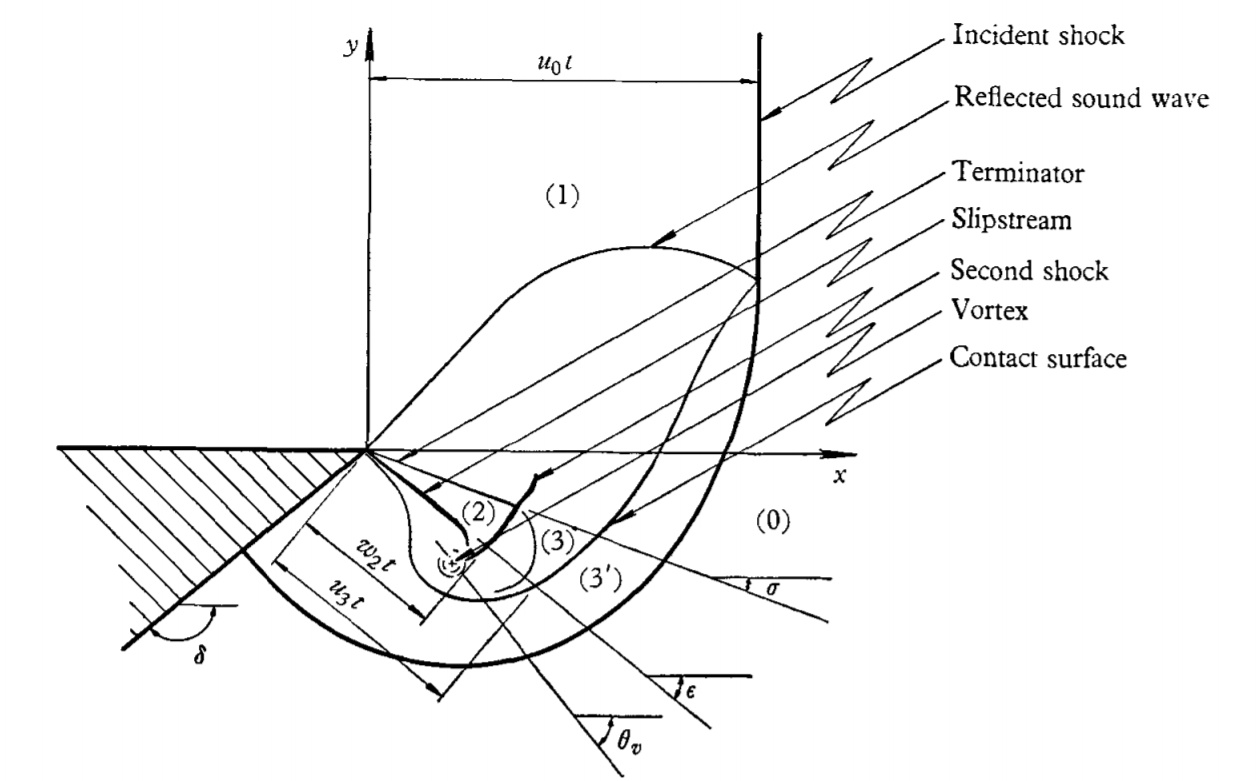
\includegraphics[scale=0.7]{fig0.PNG}
%\caption{Features of the diffraction pattern \cite{skews1967}}
%\label{fig:0}
%\end{figure}
In the next stage of jet evolution, a vortex ring is generated by the roll-up of the shear layer due to Kelvin-Helmholtz type instabilities along the slipstream at the nozzle lip \cite{elder1952experimental,dora2014role}. Kelvin-Helmholtz instabilities exist within the shock as a result of external perturbations (inhomogeneities in the flow) producing oscillations in the vortex sheet separating fluids with different flow characteristics. This structure propagates down the jet axis, and is simultaneously accompanied by the translation of a curved barrel shock formed initially at the nozzle lip. This instigates the formation of a curved Mach disk for a ratio of the nozzle exit to free-stream pressure exceeding $2.06$ \cite{matsuda1987numerical}. MORE ON MACH DISK

A triple point occurs between the leading edge of the barrel shock, the second shock, and the Mach disk. Given a sufficiently strong jet, a slip surface is generated downstream of the triple point. The first shock cell is formed in the third stage of jet evolution which is marked by the pinch-off phenomenon of the vortex ring, and signals the start of the trailing jet phase \cite{gharib1998universal}. Separation of the vortex ring from the flow structure is driven by Kelvin-Helmholtz instabilities within the shear layer of the trailing jet \cite{zhao2000effects}. The final stage of the supersonic jet is defined by the point at which the transient jet and vortex are no longer joined and the trailing jet forms. This is accompanied by the formation of a quasi-steady shock cell in self-sustained oscillation, radiating strong pressure waves. %These four stages of jet evolution are illustrated in Figure \ref{fig:2}.
%\begin{figure}[h] 
%	\centering
%	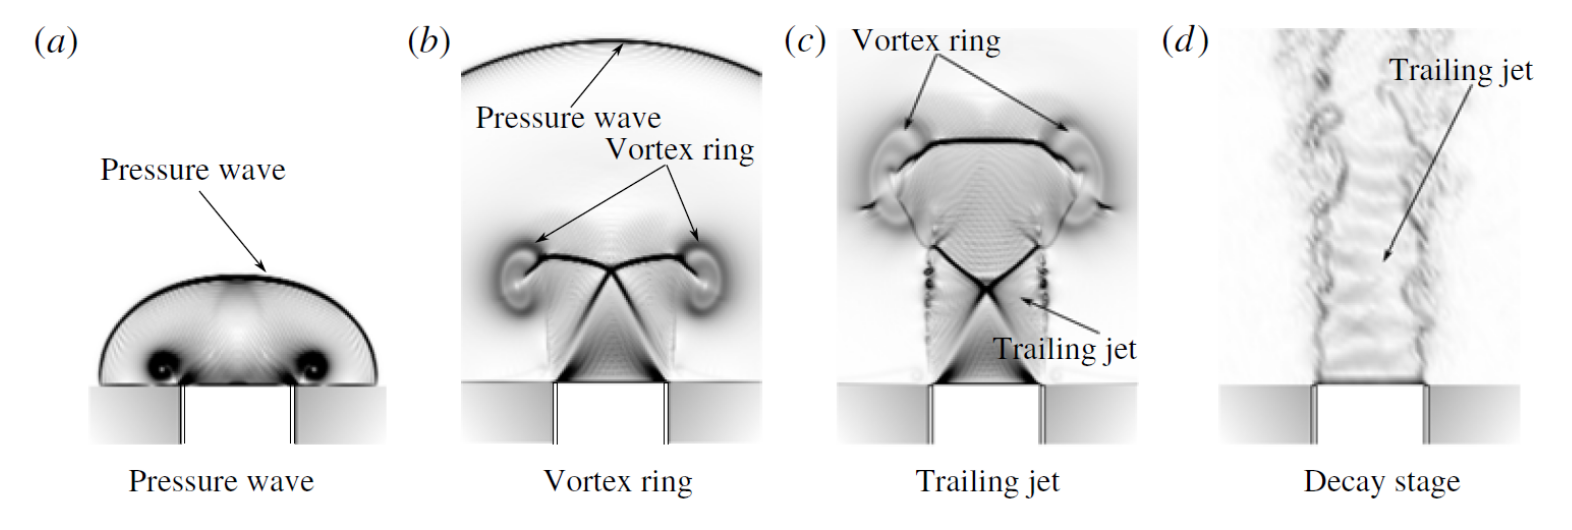
\includegraphics[scale=0.28]{fig2.png} 
%	\caption{Evolution of the transient supersonic jet. (a) Diffracting shock/Pressure
%		wave. (b) Axial translation of the vortex rings, formation of the curved shock and an unsteady Mach disk. (c) Formation of the trailing supersonic jet. (d) Decay of the trailing jet and the end of the transient jet
%		process. \cite{fernández2017}}
%	\label{fig:2}
%\end{figure}

Investigation into the high pressure plenum chamber required for PDEs currently has not been undertaken within the field. However, the flow dynamics is considered analogous to the impingement of a transient supersonic jet on a flat plate. The governing dynamics of transient jet impingment can be classified into serveral stages. The physical process is initially characterised by the reflection of the incident shock wave on the impinging plate. The reflected shock wave propargates back towards the nozzle and interacts with the approaching vortex ring. The central section of the reflected shock wave is captured by the embedded rearward-facing shock at the centre of the vortex ring, and is intensified by the opposing high-speed flow. Simultaneously, the outer section of the shock wave is diffracted by the vortex core. This process results in the formation of a toroidal shock wave which focuses in the trailing jet along the longitudinal axis of flow. The next stage of the fluid dynamics is defined by the impingement of the propagating vortex ring. Initially, as the vortex ring approaches the wall, its propagation velocity decreases and its diameter increases due to the adverse pressure gradient present \cite{szumowski2000starting}. After votex impingement the vortical flow undergoes rapid radial expansion developing a boundary layer on the surface, which slows down the flow and increases the pressure distribution over the plate. After a given duration that is dependent on the initial incident Mach number, the boundary layer separates from the plate and the flow rolls up generating a series of secondary vortices. This also occurs at the thin shear layer present between the jet flow and the exterior fluid as the region rolls up due to Kelvin-Helmholtz instabilities. This produces small interacting secondary vortex rings that propagate towards the plate \cite{minota1997shock}. Cumulative interactions between the primary and secondary wall vortex rings result in a near standing lift off of the pair. The secondary ring subsequently merges with the primary ring, and the weakened newly formed vortex ring continues to translate down the plate. %Stages of impingement are illustrated in Figure \ref{fig:4} below.

%\begin{figure}[h] 
%	\centering
%	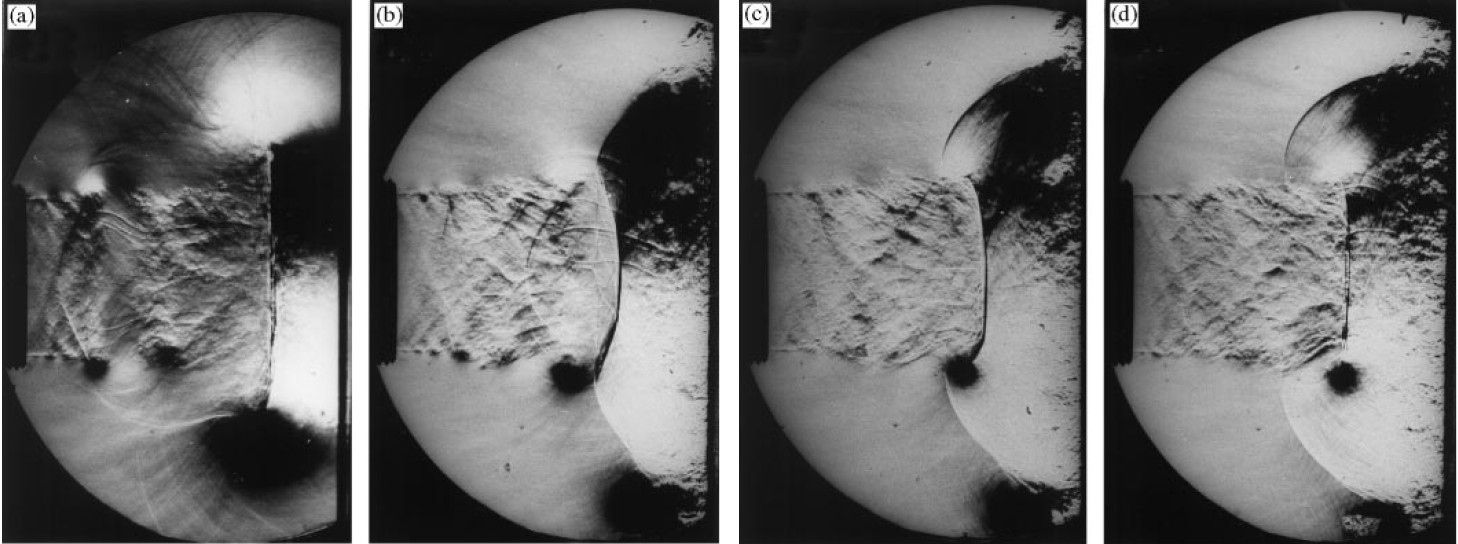
\includegraphics[scale=0.9]{fig4.PNG} 
%	\caption{Evolution of jet impingement. (a) Impingement of vortex ring. (b) Vortex ring translates down the plate. (c) Secondary vortex formation. (d) Lift-off of votex rings and dissapation. \cite{szumowski2000}}
%	\label{fig:4}
%\end{figure}
For a plate of variable angle, the lower core of the vortex ring impinges initially and generates an asymmetric set of secondary vortices. These new flow structures orbit around the main vortex, creating a temporarily thicker boundary layer at the lower end of the flow field. Again after a period of time, dependent on the incident Mach number, he boundary layer separates from the plate. This results in the vortex ring pivoting on the lower core, undergoing negligible deformation, and propergates towards the surface plate. The upper core then impinges on the plate and the upper wall vortex is generated. This new structure begins to expand radially increasing in thickness due to the remaining jet flow. While simultaneously, the lower wall vortex propagates around the outer limits of the main vortex, stops expanding, and dissipates into a thin structure. The impinging jet continues to feed into the upper section of the flow field generating wall vortices with a thicker upper core. For lower angles of plate alignment, the flow field shows an increase in overall velocity and visible curvature of the vortex ring structure during impingement. The toroidal shock wave that forms as a result of impingement propagates perpendicularly with respect to the surface \cite{mariani2013head}.  
%
The far-field noise developed by the shock wave-vortex interaction can be decomposed into three components, the sound field due to the formation and evolution of the vortex ring, the reflection shock and vortex ring interaction noise production, and the noise due to impingement of the ring on the plate. The plate-votex ring impingement noise is produced by fluctuating pressure due to the deformation and stretching of the vortex ring, formation and growth of a secondary wall vortex ring, and lifting-off of the primary-secondary vortex ring pair \cite{murugan2010characteristics}.


\newpage
\section{Experimental Methods \& Analysis Techniques}
\subsection{Shock Tube Facility}
The experiments presented were conducted in the LTRAC Supersonic Jet Facility. A schematic of the facility is shown in Figure \ref{fig:shocktube}. 

\begin{figure}[H] 
	\centering
	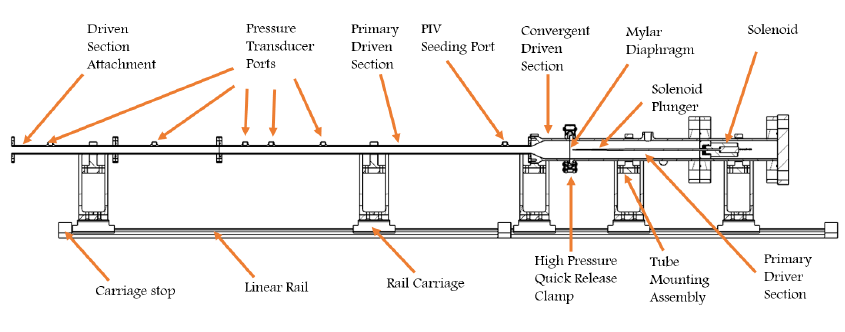
\includegraphics[width=1.05\textwidth]{fig9.PNG} 
	\caption{Shock tube facility schematic. Major parts of the
		system have been labelled.}
	\label{fig:shocktube}
\end{figure}	

The facility utilises compressed air delivered by the Monash University compressed air supply system. To produce a canonical transient supersonic jet a shock tube model is adopted \cite{john1962shock}. A typical shock tube consists of a high pressure section (driver section) and a low pressure section (driven section) separated by a diaphragm. Air enters the driver section until a desired pressure is reached, the diaphragm is then ruptured via a puncture from an actuated pin. Following the rupture, compression waves are fired down the driven section by the high pressure gas in the driver. As these compression waves travel down the tube they coalesce and form a shock wave that propagates into the test section, diffracts, and produces a transient supersonic jet. 

For the aims of this thesis, the supersonic transient jet will be studied with varied nozzle designs including a convergent, divergent and convergent-divergent configuration. Transient flow impingement will be tested via a flat plate set at $90^\circ$ to the flow. This impinging plate is set exactly at an angle of $90^\circ$ to the flow by a sequence of precisely $90^\circ$ connecting supports to the shock tube. The three nozzle designs and impingement plate will be integrated into the existing LTRAC Supersonic Jet Facility.

The relationship between the driver (4) pressure ratio and the ambient (1) pressure of the system is shown in Equation \ref{shock}, and was utilised to calculate the design incident Mach number propagating from the shock tube \cite{anderson2010fundamentals}. Figure \ref{fig:gas_relation} illustrates the effect of specific heat capacity ratio on the relation between incident Mach number and pressure ratio. Helium gas has increasingly lower pressure ratios for higher Mach numbers in comparison to air, and as a result was chosen as the driver section supply gas.

\begin{equation} \label{shock}
\frac{P_4}{P_1} = \frac{2\gamma_1M_1^2 - (\gamma_1 - 1)}{\gamma_1 + 1}\left(1 - \frac{\gamma_{4-1}}{\gamma_{1+1}}\frac{U_1}{U_4}\left(M_1 - \frac{1}{M_1}\right)\right)^{-2\gamma_4/\gamma_{4-1}}
\end{equation}

\begin{figure}[H] 
	\centering
	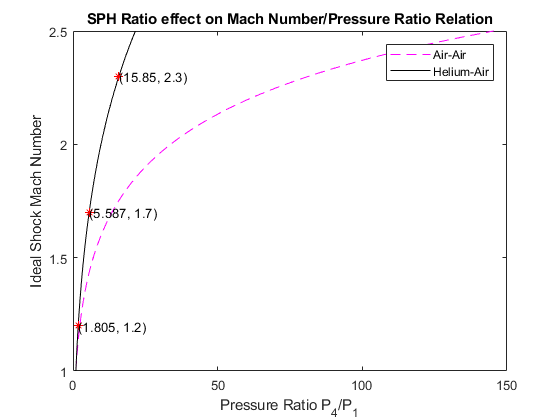
\includegraphics[scale=0.9]{fig1.png} 
	\caption{Specific Heat Capacity Ratio effect on Mach Number/Pressure Ratio Relation.}
	\label{fig:gas_relation}
\end{figure}

\subsection{Nozzle Design}
A convergent, divergent, and convergent-divergent nozzle was designed using CAD and manufactured by the Engineering department Mechanical Workshop. All three nozzle designs adopt geometry ratios implemented in the nozzles designed by Technical University of Berlin (TUB). To prevent reflecting flow and acoustic feedback loop interference, each nozzle geometry was designed with a $60^\circ$ exterior angle and a $0.5mm$ lip \cite{poldervaart1968photographic}. Each nozzle design and subsequently manufactured component is shown in Figures \ref{fig:con_noz}, \ref{fig:div_noz}, and \ref{fig:con_div_noz} below. 
 
\begin{figure}[!tbp]
  \centering
  \subfloat[CAD design (all measurements are in mm).]{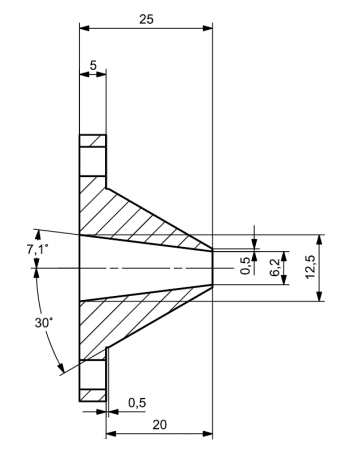
\includegraphics[width=0.4\textwidth]{convergent_cad.png}}
  \hfill
  \subfloat[Manufactured nozzle.]{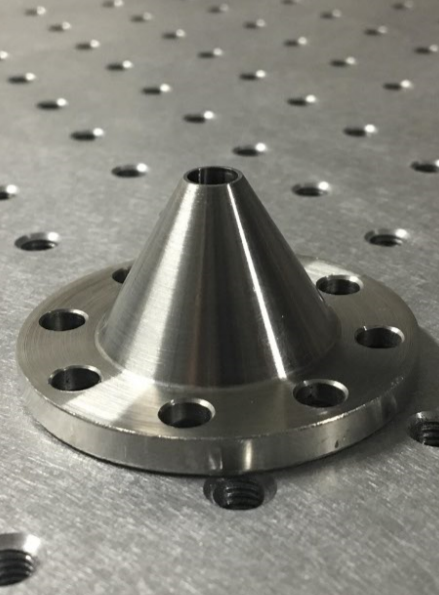
\includegraphics[width=0.4\textwidth]{con_noz.png}}
  \caption{Convergent nozzle.}
  \label{fig:con_noz}
\end{figure}

\begin{figure}[!tbp]
  \centering
  \subfloat[CAD design (all measurements are in mm).]{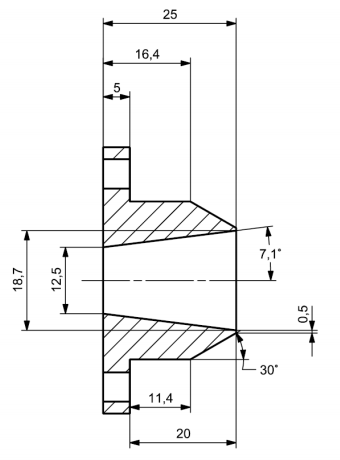
\includegraphics[width=0.4\textwidth]{divergent_cad.png}}
  \hfill
  \subfloat[Manufactured nozzle.]{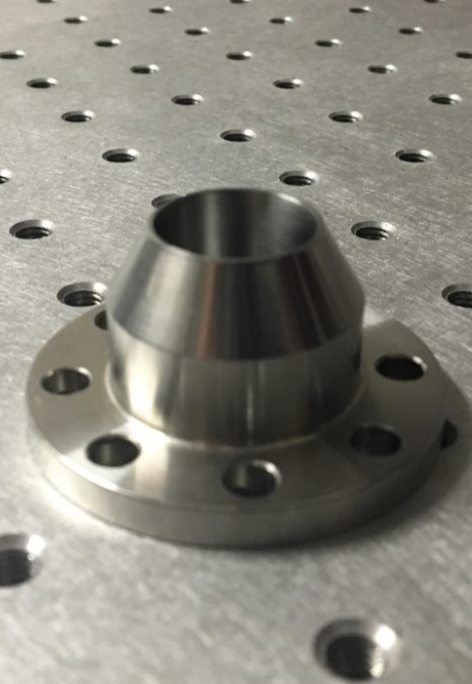
\includegraphics[width=0.4\textwidth]{div_noz.png}}
  \caption{Divergent nozzle.}
  \label{fig:div_noz}
\end{figure}

\begin{figure}[!tbp]
  \centering
  \subfloat[CAD design (all measurements are in mm).]{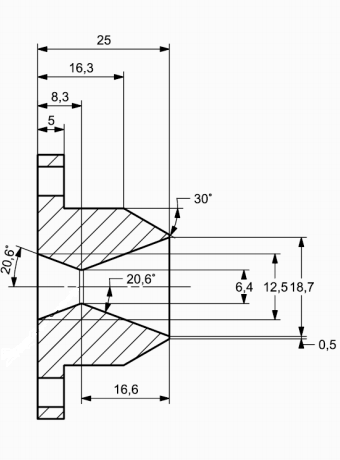
\includegraphics[width=0.4\textwidth]{con_div_cad.png}}
  \hfill
  \subfloat[Manufactured nozzle.]{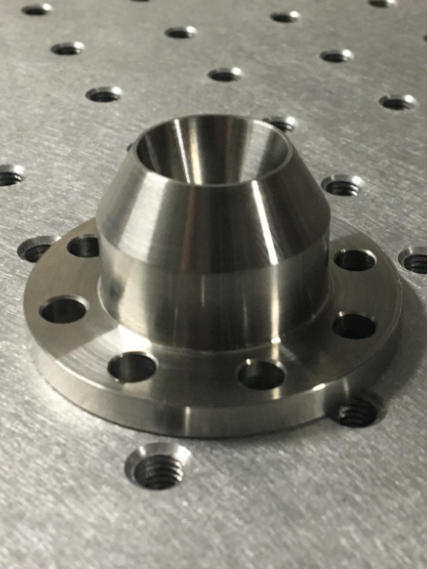
\includegraphics[width=0.4\textwidth]{con_div_noz.png}}
  \caption{Convergent-divergent nozzle.}
  \label{fig:con_div_noz}
\end{figure}

\subsection{Impingement Plate Design}
. As a result, an impingement plate distance is chosen DISTANCE AND WHY. The plate diameter is designed to appear infinite to the flow.
The impingement plate, as shown in appendix \ref{app:drawings}, is constructed such that it is $90^{\circ}$ to the direction of the flow. It mounted on rails which fix to the shock tube rig, this construction can be adjusted to 1 and 4 inner diameters. The plate is fixed to the rails such that it can be removed and replaced with another plate of alternate geometry for future research. During the evolution of a transient supersonic jet, the vortex is fully formed at approximately 3 inner diameters, from the exit for a conventional, no nozzle, shock tube \cite{mariani2013a}. As a result, an impingement plate distance is chosen below and above this limit, at 1 and 4 inner diameters, respectively. Moreover, the plate diameter is designed such that it appears infinite to the flow, to maintain consistency with the literature.
 During the evolution of a transient supersonic jet, the vortex is fully formed at approximately 3 inner diameters from the exit for a conventional, no nozzle, shock tube \cite{mariani2013head}
 
\subsection{Schlieren Imaging}
Schlieren imaging is a visualization technique that utilises the refraction of light to produce focused optical images of transparent media. Point source light is collimated and passed through a test region containing a transparent media with inhomogeneities. Light entering the test region will refract at varied degrees according to an inhomogeneous density distribution present. The light is then refocused and a knife-edge is used to partially block a fraction of incident light from the screen or camera.

The shock-driven, transient, supersonic jet is measured using a Toepler Z-type schlieren apparatus \cite{settles2001schlieren} (illustrated in Figure \ref{fig:schlieren}) with the Shimadzu HPV-1 camera. The Shimadzu has a resolution of 312 x 260 pixels and a frame rate of up to 1 million fps. 

\begin{figure}[H] 
	\centering
	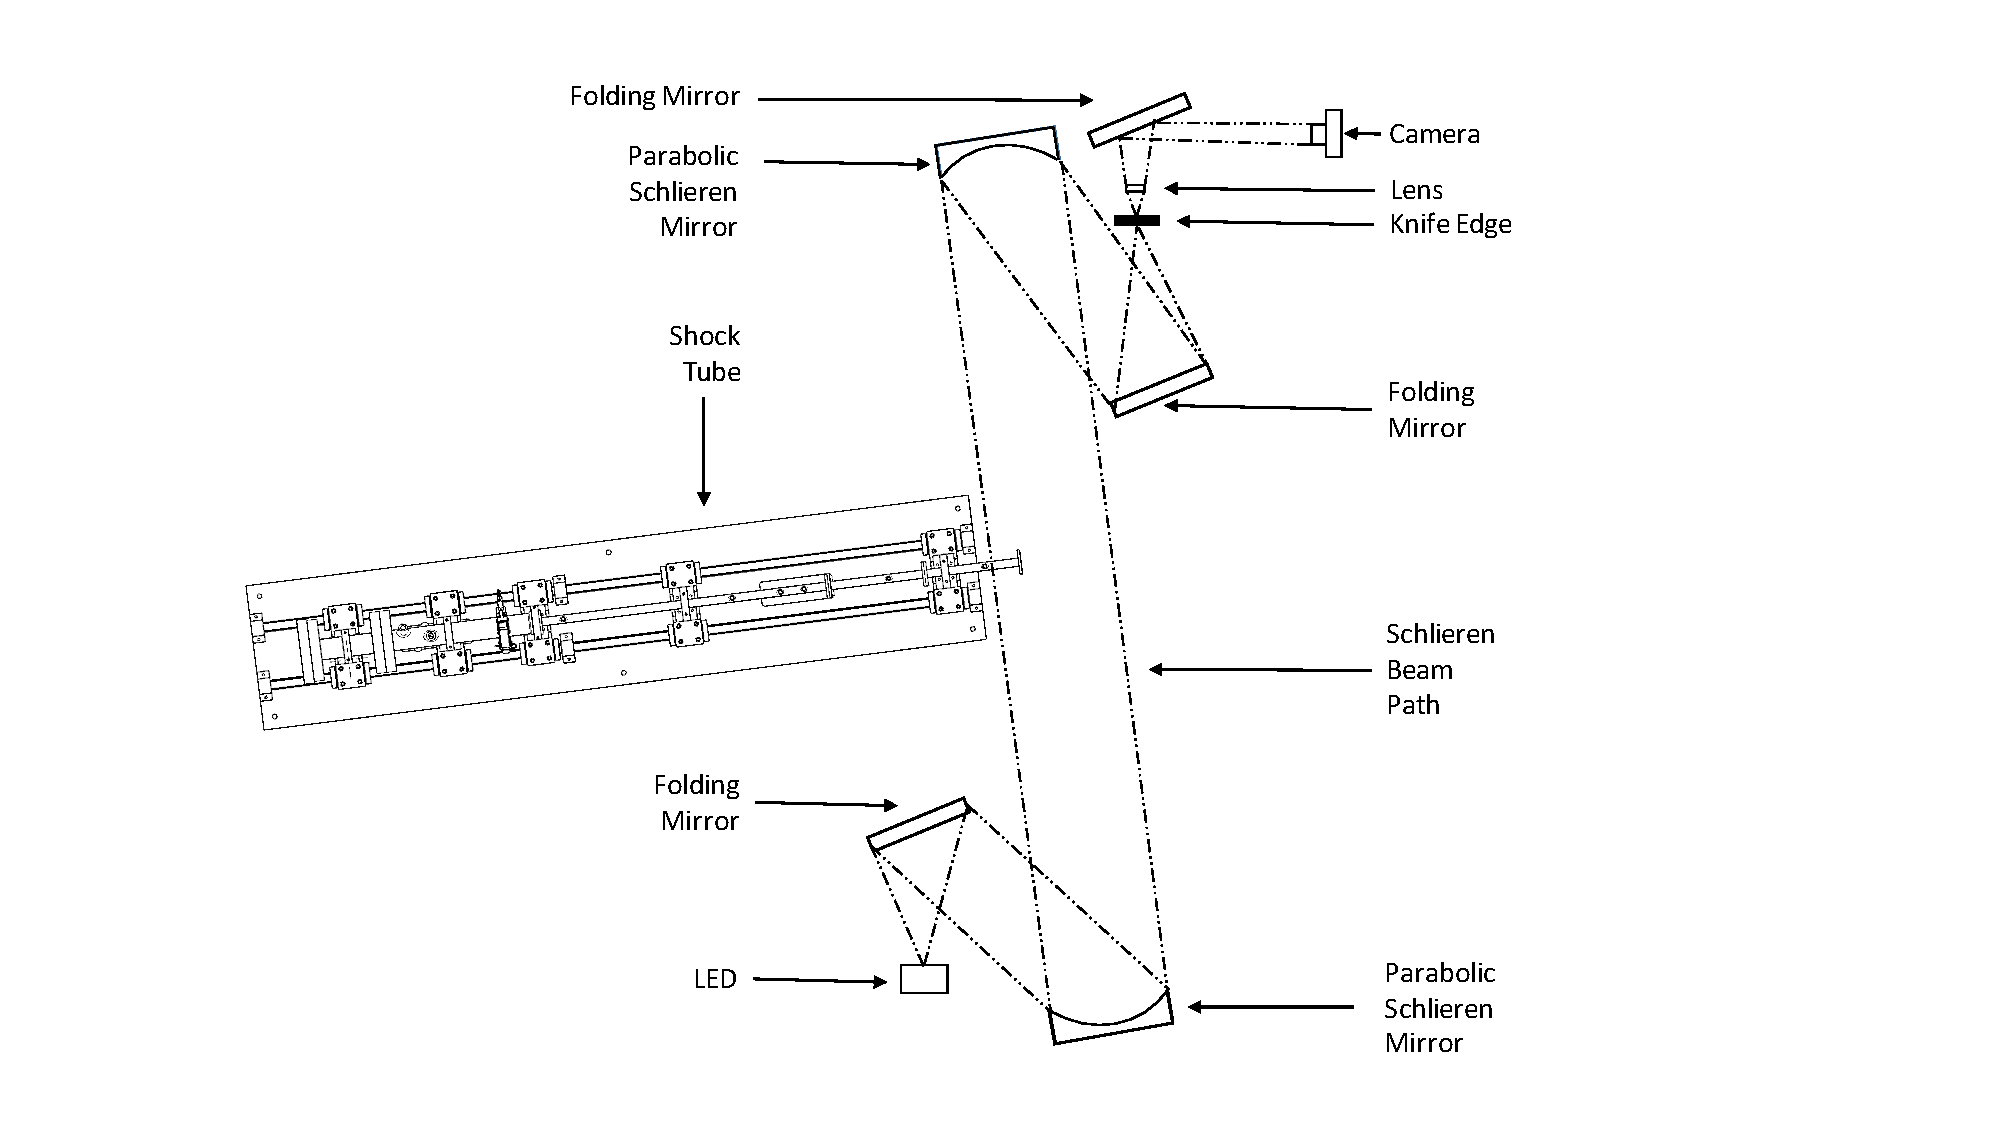
\includegraphics[width=1\textwidth]{schlieren_diagram.pdf} 
	\caption{Detail schlieren system diagram}
	\label{fig:schlieren}
\end{figure}

\subsection{Facility Development and Calibration}


\subsection{Post Processing}
Schlieren imaging produces a path integrated density gradient image that is excellent for flow visualisation but, is difficult to quantitatively extract physical parameters directly from image data. 

\subsubsection{Second Order Convolution}
the required second order image derivatives are computed by convolution with the second order derivatives of the Gaussian kernel (reference). Mathematically this means that if f denotes the image and G the normalised Gaussian, we compute
EQUATIONS
where * denotes spatial convolution, x=(x,y) denotes the pixel position, and the derivative directions i and j can be x or y. The eigenvectors and eigenvalues are computed in the algorithm from a standard second derivative Hessian matrix 

HESSIAN MATRIX

\subsubsection{Ranking Methods}
Use a normalised ranking to threshold intensity lower then the 90th percentile 

\newpage
\section{Results \& Analysis}

\newpage
\section{Discussion}

\newpage
\section{Conclusions and Recommendations}

\newpage
%\footnotesize
%\printbibliography
\bibliographystyle{ieeetr}
\bibliography{sample}

%----------------------------------------------------------------------------------------
\normalsize
\newpage

\appendix
\addcontentsline{toc}{section}{Appendix}

\section{Shock Facility} \label{app:facility}

\begin{figure}[H] 
	\centering
	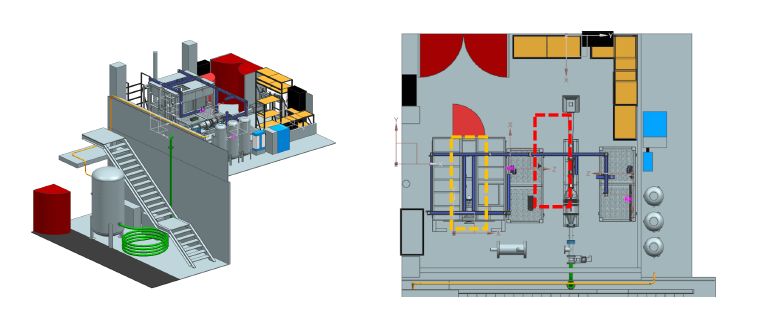
\includegraphics[width=1.05\textwidth]{fig10.PNG} 
	\caption{(Left): Isometric view of the LTRAC Shock Lab, with the shock tube facility stored under the
		shelving. (Right): Top view of the LTRAC Shock Lab, with the PIV (orange) and schlieren (red) sites
		highlighted.}
	\label{fig:10}
\end{figure}

\begin{figure}[H] 
	\centering
	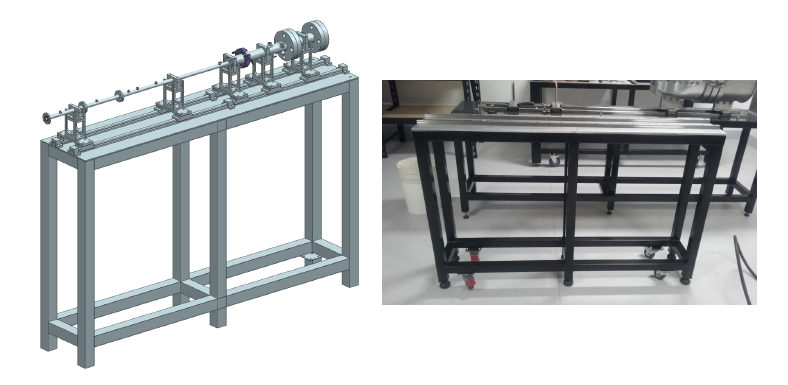
\includegraphics[width=1.05\textwidth]{fig8.PNG} 
	\caption{Isometric view of the design of the shock tube facility. (Right): Progress of the commission
		of the shock tube facility.}
	\label{fig:8}
\end{figure}

\section{Literature Comparison}
Initially, it is necessary to explore the literature and develop an understanding of the current comprehension of the flow characteristics governing supersonic transient jet impingement, and previous experimental test configurations. Section \ref{sec:background} undertakes an extensive review of previous literature, exploring the fluid dynamics and practical applications of supersonic impinging jets. Table \ref{tab1} details a summary for the research undertaken in previous literature, it's important to note all previous literature sources implement a plate diameter such that it can be considered infinite to the flow. Additionally, imaging results from the literature summarised in Table 1 is subsequently shown in appendix \ref{app:litresults}.

\begin{table}[h]
	\centering
	\caption{Literature Summary}
	\label{tab1}
	\resizebox{\textwidth}{!}{ 
		\begin{tabular}{@{}llllll@{}}
			\toprule
			Reference                                                                                                                           & \begin{tabular}[c]{@{}l@{}}Main\\ Research\\ Focus\end{tabular}                                                          & \begin{tabular}[c]{@{}l@{}}Imaging\\ Technique\end{tabular}                                            & \begin{tabular}[c]{@{}l@{}}Inner Shock\\ Tube\\ Diameter\end{tabular} & \begin{tabular}[c]{@{}l@{}}Incident\\ Mach\\ Number\end{tabular} & \begin{tabular}[c]{@{}l@{}}Impingement\\ Plate Distance\\ (inner diameter)\end{tabular}   \\ \midrule
			\multicolumn{1}{|l|}{\cite{minota1997shock}}                                                                                              & \multicolumn{1}{l|}{\begin{tabular}[c]{@{}l@{}}Shock-vortex \\ interaction in \\ the flow field\end{tabular}}            & \multicolumn{1}{l|}{Shadowgraph}                                                                       & \multicolumn{1}{l|}{40mm}                                             & \multicolumn{1}{l|}{1.35}                                        & \multicolumn{1}{l|}{0.4di}                                                                \\ \midrule
			\multicolumn{1}{|l|}{\cite{szumowski2000starting}}                                                                                              & \multicolumn{1}{l|}{\begin{tabular}[c]{@{}l@{}}Sound generation \\ upon impingement\end{tabular}}                        & \multicolumn{1}{l|}{Schlieren}                                                                         & \multicolumn{1}{l|}{65mm}                                             & \multicolumn{1}{l|}{1.14}                                        & \multicolumn{1}{l|}{2di}                                                                  \\ \midrule
			\multicolumn{1}{|l|}{\cite{murugan2010characteristics}}                                                                                              & \multicolumn{1}{l|}{\begin{tabular}[c]{@{}l@{}}Noise due to shock-\\ vortex interaction \\ and impingement\end{tabular}} & \multicolumn{1}{l|}{\begin{tabular}[c]{@{}l@{}}High-speed\\ smoke flow\\ visualisations.\end{tabular}} & \multicolumn{1}{l|}{64mm}                                             & \multicolumn{1}{l|}{1.31 - 1.55}                                 & \multicolumn{1}{l|}{4.7di}                                                                \\ \midrule
			\multicolumn{1}{|l|}{\cite{thangadurai2012experimental}}                                                                                              & \multicolumn{1}{l|}{\begin{tabular}[c]{@{}l@{}}Vortex ring\\ impingement\end{tabular}}                                   & \multicolumn{1}{l|}{\begin{tabular}[c]{@{}l@{}}High-speed\\ smoke flow\\ visualisations.\end{tabular}} & \multicolumn{1}{l|}{64mm}                                             & \multicolumn{1}{l|}{1.31 - 1.85}                                 & \multicolumn{1}{l|}{4.7di}                                                                \\ \midrule
			\multicolumn{1}{|l|}{\cite{mariani2013head}}                                                                                              & \multicolumn{1}{l|}{\begin{tabular}[c]{@{}l@{}}Vortex ring\\ impingement\end{tabular}}                                   & \multicolumn{1}{l|}{Schlieren}                                                                         & \multicolumn{1}{l|}{30mm}                                             & \multicolumn{1}{l|}{1.61}                                        & \multicolumn{1}{l|}{\begin{tabular}[c]{@{}l@{}}1.66di, \\ 3.33di, \\ 5.00di\end{tabular}} \\ \bottomrule
		\end{tabular}}
	\end{table}

\section{Shock Relations} \label{app:shock}
In this section, the relationship between the pressure of the flow behind the leading shock and the ambient pressure will be derived. Figure \ref{fig:shock} details pressure, temperature, and velocity relations for the shock tube.

\begin{figure}[H]
	\centering
	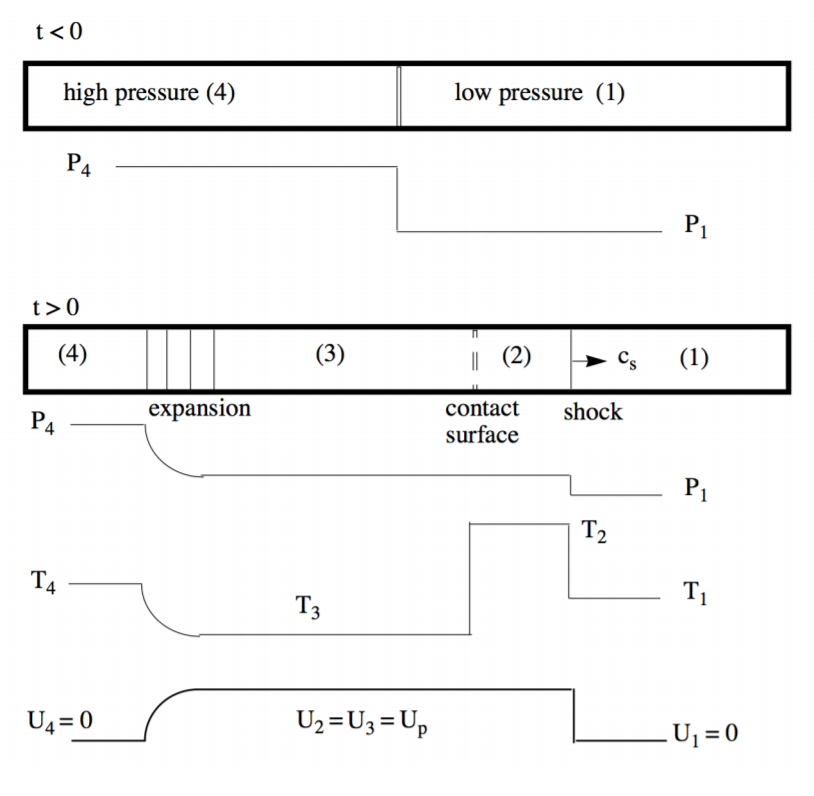
\includegraphics[scale=0.5]{figshock.png} 
	\caption{Shock tube flow regions: Region 1 is the flow ahead of the primary shock, region 2 is between contact surface and primary shock, region 3 is between tail of the expansion fan and contact surface, region 4 is ahead of the leading expansion wave \cite{cantwell2017}.}
	\label{fig:shock}
\end{figure}

In the following we will combine the results for expansion waves with normal shock relations to derive the so-called shock tube equation. The conditions at the contact surface are:
\begin{equation}
	P_2 = P_3 
\end{equation}
\begin{equation}
	U_2 = U_3 = U_p.
\end{equation}
\begin{center}
	where $U_2$ is the speed of the slug of gas set into motion by the opening of the diaphragm.
\end{center}
This is the effective piston speed of the fluid released by the diaphragm.

In a frame of reference moving with the shock wave the gas velocities are
\begin{equation}
U'_1 = -c_s
\end{equation}
\begin{equation}
U'_2 = -c_s + U_p
\end{equation}
and the shock jump conditions are

\begin{equation}
\frac{U'_2}{U'_1} = \frac{1+\frac{\gamma_1-1}{2}M_1^2}{\frac{\gamma_1+1}{2}M_1^2} 
\end{equation}
\begin{equation}
\frac{P_2}{P_1} = \frac{\gamma_1M_1^2-\frac{\gamma_1-1}{2}}{\frac{\gamma_1+1}{2}} 
\end{equation}
\begin{center}
	where $M_1 = c_s/a_1 = -U'_1/a_1$. Using the first relation, Equation 5 above, we can write
\end{center}

\begin{equation}
\frac{U'_2 - U'_1}{U'_1} = \frac{1 + \frac{\gamma_1-1}{2}M_1^2}{\frac{\gamma_1+1}{2}M_1^2} - 1 = \frac{1 - M_1^2}{\frac{\gamma_1+1}{2}M_1^2}
\end{equation}

The piston velocity is

\begin{equation}
U_p = U'_2 - U'_1 = U'_1\left(\frac{1 - M_1^2}{\frac{\gamma_1+1}{2}M_1\frac{-U'_1}{a_1}}\right) = a_1\left(\frac{M_1^2 - 1}{\frac{\gamma_1+1}{2}M_1}\right) 
\end{equation}

Note that $U_p$ is positive. Using the second relation, Equation 5, Equation 8 can be expressed in terms of the shock pressure ratio as 

\begin{equation}
U_p = a_1\left(\frac{P_2}{P_1} - 1\right)\left(\frac{2}{\gamma_1(\gamma_1 + 1)(P_2/P_1) + \gamma_1(\gamma_1 - 1)}\right)^{1/2}
\end{equation}

Equation 9 is the expression for the piston velocity derived using normal shock theory. Now lets work out an expression for the piston velocity using isentropic expansion theory. The velocity behind the expansion is

\begin{equation}
U_3 = U_p = \frac{2a_4}{\gamma_4 - 1}\left(1 - \frac{P_3}{P_4}^{\frac{\gamma_4 - 1}{2\gamma_4}}\right)
\end{equation}

Equate 9 and 10.

\begin{equation}
a_1\left(\frac{P_2}{P_1} - 1\right)\left(\frac{2}{\gamma_1(\gamma_1 + 1)(P_2/P_1) + \gamma_1(\gamma_1 - 1)}\right)^{1/2} = \frac{2a_4}{\gamma_4 - 1}\left(1 - \left(\frac{P_3}{P_2}\frac{P_2}{P_1}\frac{P_1}{P_4}\right)^{\frac{\gamma_4 - 1}{2\gamma_4}}\right)
\end{equation}

Using the following identity

\begin{equation}
\frac{P_3}{P_4}=\frac{P_3}{P_2}\frac{P_2}{P_1}\frac{P_1}{P_4}
\end{equation}

and noting that $P_3/P_2 = 1$ solve Equation 10 for $P_4/P_3 = 1$, substituting in $P_2/P_1$ from Equation 6. Simplifying, the result is the basic shock tube equation

\begin{equation}
\frac{P_4}{P_1} = \frac{2\gamma_1M_1^2 - (\gamma_1 - 1)}{\gamma_1 + 1}\left(1 - \frac{\gamma_{4-1}}{\gamma_{1+1}}\frac{U_1}{U_4}\left(M_1 - \frac{1}{M_1}\right)\right)^{-2\gamma_4/\gamma_{4-1}}
\end{equation}
And given the specific gas information, for the driver helium, $\gamma_4 = 1.667$, and the driven air, $\gamma_1 = 1.4$. Taking the ambient air temperature $T_1 = 273.15K$, the relation in equation 13 can be shown in the Figure \ref{fig:15}. This figure highlights the relationship between the driver pressure ratio at 4, and the ambient pressure at 1, for a design incident Mach number. The figure also illustrates the reduced pressure ratio benefit of using a helium to air experiment in comparison to a air to air experiment. 
	

\end{document}
